\documentclass{article}

\usepackage[T1]{fontenc}
\usepackage[utf8]{inputenc}
\usepackage{graphicx}
\usepackage{booktabs, siunitx}
\usepackage{tikz}
\usepackage{tikz-qtree}
\usepackage{pifont}
\usepackage[margin=0.90in]{geometry}
\usepackage{etoolbox,titling}
\usepackage{enumitem}
\usepackage{fancyhdr}
\usepackage{soulutf8}
\usepackage{tcolorbox}
\tcbuselibrary{skins}

\definecolor{boxTitle}{HTML}{fff79a}
\definecolor{boxBackground}{HTML}{fffce0}
\definecolor{boxFrame}{HTML}{f1e2b8}


\definecolor{boxTitle2}{HTML}{b3ffda}
\definecolor{boxBackground2}{HTML}{e6f2ff}
\definecolor{boxFrame2}{HTML}{b3d7ff}

\definecolor{boxTitle3}{HTML}{ff794d}
\definecolor{boxBackground3}{HTML}{ffe6e6}
\definecolor{boxFrame3}{HTML}{ffb399}

\definecolor{boxTitle4}{HTML}{d7d7c1}
\definecolor{boxBackground4}{HTML}{ebebe0}
\definecolor{boxFrame4}{HTML}{c3c3a2}


\tcbset{box1/.style={
    enhanced, fonttitle=\bfseries,
    colback=boxBackground, colframe=boxFrame,
    coltitle=black, colbacktitle=boxTitle,
    attach boxed title to top left={xshift=0.3cm,
                                    yshift*=-\tcboxedtitleheight/2}
  }
}
\newtcolorbox{box1}[1][]{box1, #1}

\tcbset{box2/.style={
    enhanced, fonttitle=\bfseries,
    colback=boxBackground2, colframe=boxFrame2,
    coltitle=black, colbacktitle=boxTitle2,
    attach boxed title to top left={xshift=0.3cm,
                                    yshift*=-\tcboxedtitleheight/2}
  }
}
\newtcolorbox{box2}[1][]{box2, #1}

\tcbset{box3/.style={
    enhanced, fonttitle=\bfseries,
    colback=boxBackground3, colframe=boxFrame3,
    coltitle=black, colbacktitle=boxTitle3,
    attach boxed title to top left={xshift=0.3cm,
                                    yshift*=-\tcboxedtitleheight/2}
  }
}
\newtcolorbox{box3}[1][]{box3, #1}

\tcbset{box4/.style={
    enhanced, fonttitle=\bfseries,
    colback=boxBackground4, colframe=boxFrame4,
    coltitle=black, colbacktitle=boxTitle4,
    attach boxed title to top left={xshift=0.3cm,
                                    yshift*=-\tcboxedtitleheight/2},
    boxed title style={
      before upper=\hspace*{0.5cm},
      overlay={
       \node at ([xshift=0.1cm]frame.west)
         {\includegraphics[scale=0.65]{bc-loupe}};
      }
    }
  }
}

\newtcolorbox{box4}[1][]{box4, #1}

\pagestyle{fancy}
\fancyhf{}
\rhead{Check My Blob}
\lhead{Traccia presentazione}
\rfoot{Pagina \thepage}
\lfoot{Bioinformatica - A.A. 2021/22}
\usetikzlibrary{trees}
\tikzstyle{every node}=[draw=black,thick,anchor=west]


\begin{document}
\newcommand\tab[1][0.3cm]{\hspace*{#1}}


\begin{titlepage}
    \begin{center}
        \vspace*{1cm}
            
        \Huge
        \textbf{Check My Blob}\\
        \LARGE
        \textbf{Come funziona? Pipeline di lavoro.}
            
        \vspace{0.5cm}
        \LARGE
        Laboratorio di Bioinformatica, Modulo 2 - Presentazione
            
        \vspace{1.5cm}
            
        \textbf{Chiara Solito}

        \vspace{0.8cm}

            
        \Large
        Corso di Laurea in Bioinformatica\\
        Università degli studi di Verona\\
        A.A. 2021/22
            
    \end{center}
\end{titlepage}

\newpage
\thispagestyle{empty}
\section{Com'è stato costruito l'algoritmo Check My Blob?}
Partiamo dalla collezione dei dati, per poi osservare come sono stati raggruppati i ligandi a partire dai dati raccolti e poi com'è stato addestrato il modello.
\subsection{Data Collection}
Il training set partiva da tutte le entry PDB scaricate il 19 Gennaio 2020. Dopo una necessaria "pulizia" dei dati, il training set finale consisteva in ligandi derivati da esperimenti di diffrazione a raggi X con almeno 4,0 Å di risoluzione.
\subsection{Clustering dei Ligandi}
Il passo successivo è stato clusterizzare i ligandi.\\Diversi ligandi sono indistinguibili dalla sola densità elettronica. Ad esempio, per la maggior parte degli intervalli di risoluzione, è estremamente difficile distinguere tra 6, 7 o 8 elettroni (carbonio, azoto, ossigeno) 
o distinguere tra legami singoli, doppi o tripli in alcune configurazioni. Per migliorare la robustezza dell'algoritmo di classificazione, per Check My Blob è stato deciso di raggruppare i ligandi in base alla forma prevista dalla loro densità elettronica derivata 
dalle loro definizioni chimiche. Vale a dire, che si è considerata la connettività dell'atomo, la chiralità e le differenze significative nel numero di elettroni ma si è ignorato il tipo di atomo e l'ordine di legame in qualche equivalente configurazione. La procedura di raggruppamento è stata la seguente:
\begin{enumerate}
  \item Raggruppare le molecole facendo corrispondere il numero di atomi, anelli, e anelli aromatici;
  \item Raggruppare per connettività (abbinando le sottostrutture, utilizzando atomi generici e legami generici);
  \item Controllare se la chiralità di tutte le combinazioni corrispondenti convalida;
  \item Verificare se i modelli SMART corrispondono a posizioni equivalenti;
  \item Controllare se gli atomi equivalenti sono nello stesso gruppo di numeri atomici.
\end{enumerate}
\subsection{Modello}
Il modello di classificazione primario (GBM) è stato addestrato a riconoscere i 219 gruppi di ligandi più popolari (cluster). Questo numero è stato raggiunto limitando la formazione alle classi con almeno 100 esempi nel set di formazione. 
Tutti i ligandi che non erano in quei 219 gruppi sono stati etichettati come una classe separata chiamato "rara". Quando il modello di classificazione primario prevede "raro", l'esempio viene ulteriormente elaborato da un secondario modello (algoritmo 1-NN) addestrato solo su ligandi nel gruppo "raro".
\subsection{Validazione del modello}
Successivamente vi è stata una validazione del modello.
\begin{center}
  \begin{tabular}{c|c|c}
  \toprule
    & 10-fold CV & Hold out Set\\
    \midrule
    Ligand instances & 696 887 & 17 150 \\
    Mean resolution (Å) & 2.2 & 2.5 \\
    Accuracy (\%) & 71.2(9) & 58.9 \\
    Top-5 accuracy (\%) & 90.7(5) & 87.2 \\
    Top-10 accuracy (\%) & 94.9(2) & 92.5 \\
    Micro-averaged recall (\%) & 71.2(9) & 58.9 \\
    Micro-averaged precision (\%) & 69.3(11) & 62.7 \\
    Micro-averaged F1 (\%) & 69.3(11) & 55.7 \\
    Cohen's kappa (\%) & 64.6(12) & 46.2 \\
    \bottomrule
  \end{tabular}
\end{center}
L'hold out set era più impegnativo perché conteneva una risoluzione inferiore strutture di soluzione, ma i risultati sono comunque superiori a quelli segnalati per ligandi non clusterizzati con almeno due atomi di idrogeno.

\section{Come funziona la pipeline di lavoro?}
Stabilito il modo in cui è stato creato l'algoritmo Check My Blob vediamo cosa succede quando effettivamente si utilizza il web server.
\paragraph*{Fase di apprendimento:} I blob non interpretati vengono “tagliati” dalle mappe di densità elettronica generate tramite la sezione “polymer-only-portion” di PDB.\\
I blob vengono trovati automaticamente analizzando tutti i picchi di densità elettronica positivi all'interno della mappa Fo-Fc. Per mitigare il problema dei ligandi divisi in più blob, il sistema rileva i massimi locali e scheletizza la densità elettronica all'interno dell'isosuperficie di ciascun blob e 
combina i blob adiacenti se la distanza tra i massimi locali o i nodi dello scheletro è inferiore a 2,15 Å. Infine, tutti i frammenti di densità elettronica nell'isosuperficie del blob che si sovrappongono all'isosuperficie degli atomi del biopolimero modellato vengono ritagliati dal blob. In pratica, CheckMyBlob è in grado di rilevare ligandi costituiti da decine di candidati blob.
\paragraph*{Descrizione del blob:} Ogni blob è descritto tramite un set di feature numeriche, che sono date in pasto all'algoritmo di machine learning (un classificatore). 
\paragraph*{Classificazione:} Il classificatore crea una funzione (un modello di classificazione) che predice i migliori ligandi basandosi sulle feature numeriche.

\section{Performance e attendibilità dei risultati}
Anche se le istanze del ligando utilizzate per l'addestramento sono selezionate in base a diversi criteri di qualità, ogni previsione di CheckMyBlob dovrebbe essere trattata come un suggerimento che necessita di ulteriori indagini.\\
La predizione si basa sulla mappa di densità degli elettroni, mentre la conoscenza dei ligandi che potrebbero essere presenti nel cristallo è basata su:
\begin{itemize}
  \item condizioni di cristallizazione
  \item componenti del protein buffer
  \item componenti aggiuntive
  \item componenti che potrebbero essere stati eliminati durante la purificazione proteica
  \item tutte le reazioni chimiche tra questi
\end{itemize}

L'affidabilità di una previsione concreta può essere misurata dalla certezza della previsione (probabilità).\\
Ogni previsione del server è accompagnata da una probabilità percentuale che il server abbia ragione. L'istogramma e il line plot di seguito mostrano la frequenza con cui il server è stato corretto per un determinato livello di certezza, in termini di valori assoluti e relativi. Entrambi i grafici mostrano che le previsioni con maggiore certezza sono in realtà molto probabili, mentre le previsioni con valori di certezza inferiori hanno una maggiore probabilità di essere errate.
\begin{center}
  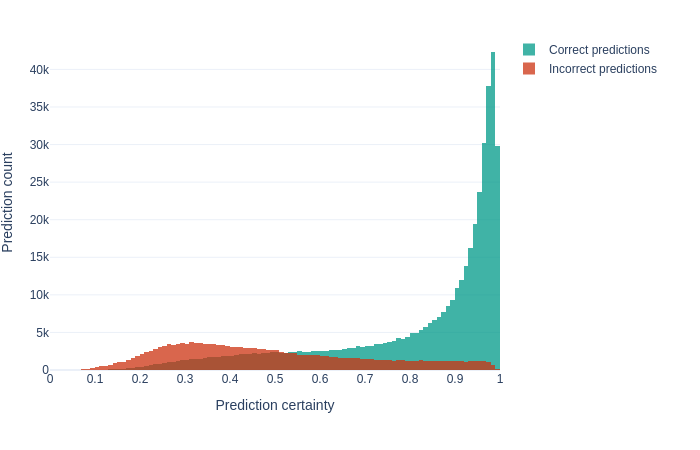
\includegraphics[width=1\textwidth]{figures/Istogramma.png}
\end{center}

\begin{center}
  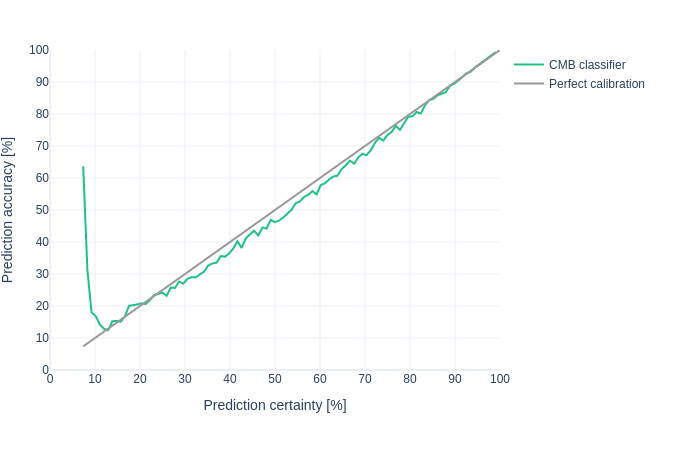
\includegraphics[width=1\textwidth]{figures/LinePlot.png}
\end{center}

\end{document}